%#########################################################################################
%#------- PREAMBLE ----------------------------------------------------------------------#
%#########################################################################################

\documentclass[11pt,twocolumn,a4paper,twoside]{article}

\usepackage{amsmath, amsthm, amscd, amsfonts, amssymb, mathtools}

%\usepackage[top=15mm, bottom=15mm, left=15mm, right=15mm, paperwidth=19cm,paperheight=26.5cm]{geometry}
%\usepackage[top=15mm, bottom=15mm, outer=15mm, inner=15mm, paperwidth=20cm,paperheight=26.5cm]{geometry}
\usepackage{geometry}
 \geometry{
 a4paper,
 total={210mm,297mm},
 left=23mm,
 right=23mm,
 top=30mm,
 bottom=25mm,
 }
\usepackage{setspace}
\usepackage{graphicx}
\usepackage{wasysym}
\usepackage{framed}
\usepackage{xcolor}
\usepackage[hyphens]{url}
\usepackage{flushend}
\usepackage[a4,center,noinfo]{crop}
%\usepackage[compact]{titlesec}
%\usepackage[rawfloats=true]{floatrow}
\usepackage{balance}
%\usepackage{multicol}
%\usepackage{scrextend}
%\deffootnote[0.5em]{1em}{1em}{\scriptsize\thefootnotemark\enskip}

\usepackage{manyfoot}
\usepackage{bussproofs}

\makeatletter
\def\@makefnmark{\hbox{\@textsuperscript{\@thefnmark}}}
\renewcommand\@makefntext[1]{%
\let\@textsuperscript\relax    \parindent 1em%
    \noindent
    \hb@xt@0.8em{\hss\@makefnmark}\ {\scriptsize #1}}
\makeatother


\usepackage{fancyhdr}

\usepackage{atbegshi}
\usepackage{textpos}
\usepackage{rotating}
%\usepackage{eso-pic}
%\usepackage{background}

%\usepackage{marginnote}

\usepackage{tikz}
%%%%%%%%%%%%%%
\usetikzlibrary{decorations.pathreplacing, positioning, arrows.meta}
%%%%%%%%%%%%%%%
\usepackage{enumitem}
%\setlength{\parskip}{0em} % تنظیم فاصله بین پاراگراف‌ها
%\setlength{\parindent}{0em}

\usepackage[documentdirection=righttoleft]{xepersian}
\settextfont[Scale=1]{XB Yagut}
% \setdigitfont[Scale=1]{XB Yagut}

%\settextfont[Scale=1]{B Lotus}
%\setdigitfont[Scale=1]{B Lotus}
\setlatintextfont[Scale=0.9]{Times New Roman}
%\settextfont{Times New Roman}
\defpersianfont\Titre[Scale=1]{XB Titre}
\defpersianfont\Zar[Scale=1]{XB Zar}
\defpersianfont\Niloofar[Scale=0.9]{XB Niloofar}

\usepackage{perpage}
\MakePerPage[1]{footnote}

\linespread{1.48}
\setlength{\columnsep}{6.5mm}

\newcommand{\keyword}[1]{\textbf{واژه‌های کلیدی:} #1}


\pagestyle{fancyplain}% <- use fancyplain instead fancy
\fancyhf{}

\usepackage{fancyhdr}
\pagestyle{fancy}
%%%%%%%%%%%%%%%%%%%%%%%%%%%% The paper headers
\fancyhead[LO,RE]{\thepage \vspace{2mm}}
\fancyhead[RO]{
صوری‌سازی ترجمه حذف وابستگی در سیستم‌های نوع محض لایه‌ای / حسین مددی و مجید علی‌زاده
\vspace{2mm}
}% odd page header and number to right top
\fancyhead[LE]{فصلنامه علمی، علوم رایانشی، سال یازدهم، شماره 43، زمستان 1405
\vspace{2mm}
}%Even page header and number at left top
\fancyfoot[L,R,C]{}
\renewcommand{\headrulewidth}{0.4pt}% disable the underline of the header part
\fancypagestyle{firstpage}{%
  \lhead{\LR{\scriptsize DOR: X}\\
  \vspace{-2mm}\noindent\rule{0.45\linewidth}{0.4pt}\\
  \LR{\scriptsize DOI: Y}\\
  {\scriptsize
زمستان 1405، دوره 11، شماره 4، پیاپی 43
  }
  }
  \rhead{}
  \lfoot{\thepage}
  \renewcommand{\headrulewidth}{0pt}% disable the underline of the header part
}

\theoremstyle{definition}
\newtheorem{definition}{تعریف}[section]
\renewcommand{\thedefinition}{\thesection.\arabic{definition}}


\theoremstyle{theorem}
%\newtheorem{theorem}[definition]{قضیه}
\newtheorem{theorem}{قضیه}[section]
\renewcommand{\thetheorem}{\thesection.\arabic{theorem}}


\theoremstyle{definition}
%\newtheorem{lemma}[definition]{لم}
\newtheorem{lemma}{لم}[section]
\renewcommand{\thelemma}{\thesection.\arabic{lemma}}


\theoremstyle{definition}
%\newtheorem{proposition}[definition]{گزاره}
\newtheorem{proposition}{گزاره}[section]
\renewcommand{\theproposition}{\thesection.\arabic{proposition}}


\theoremstyle{definition}
%\newtheorem{corollary}[definition]{نتیجه}
\newtheorem{corollary}{نتیجه}[section]
\renewcommand{\thecorollary}{\thesection.\arabic{corollary}}


\theoremstyle{definition}
%\newtheorem{remark}[definition]{ملاحظه}
\newtheorem{remark}{ملاحظه}[section]
\renewcommand{\theremark}{\thesection.\arabic{remark}}
%\theoremstyle{definition}
%\newtheorem{example}[definition]{مثال}

\theoremstyle{definition}
\newtheorem{example}{مثال}[section]
\renewcommand{\theexample}{\thesection.\arabic{example}}



\newcommand{\bk}{\mathbf{K}}
\newcommand{\cf}{\mathbf{CFE}}
\newcommand{\atom}{\mathbf{Atom}}
\newcommand{\agt}{\mathbf{Agt}}
\newcommand{\act}{\mathbf{Act}}
\newcommand{\norm}{\mathbf{Norm}}
\newcommand{\ec}{\mathbf{EC}}
\newcommand{\bG}{\mathbf{Goal}}
\newcommand{\hp}{\mathbf{HP}}
\newcommand{\mm}{\mathbf{Imm}}
\newcommand{\nq}{\mathbf{Inq}}
\newcommand{\cha}{\mathbf{CHA}}
\newcommand{\guilt}{\mathbf{Guilt}}
\newcommand{\shame}{\mathbf{Shame}}
\newcommand{\adv}{\mathbf{Advantage}}
\newcommand{\envy}{\mathbf{Envy}}
\newcommand{\regret}{\mathbf{Regret}}
\newcommand{\Social}{\mathbf{Social}}

\newcommand{\resizedalign}[1]{%
  \[
  \resizebox{\columnwidth}{!}{$
    \begin{aligned}
      #1
    \end{aligned}
  $}
  \]
}

\newcommand{\filename}[1]{\lr{\texttt{#1}}}
\newcommand{\varname}[1]{\lr{\texttt{\footnotesize\detokenize{#1}}}}

\usepackage{listings}
\usepackage{xcolor}

\lstdefinelanguage{Rocq}{
    morekeywords={
        Module, Type, End, Parameter, Import,
        Require, Include, Axiom, forall,
        Prop, nat, Type, exists,
        Definition, Theorem, Qed, Proof, Fixpoint, with, match, Inductive,
        end
    },
    sensitive=true,
    morecomment=[n]{(*}{*)},
    morestring=[b]"
}

\lstdefinestyle{Rocqstyle}{
    language=Rocq,
    basicstyle=\ttfamily\footnotesize,
    keywordstyle=\color{blue!70!black},
    commentstyle=\color{gray},
    numbers=none,
    frame=none,
    breaklines=true,
    breakatwhitespace=false,
    showstringspaces=false,
    tabsize=2,
    captionpos=b,
    columns=fullflexible,
    keepspaces=true
}

\usepackage{caption}
\captionsetup{
    font=small,
    labelfont=bf
}

%\makeatletter
%\renewcommand{\@seccntformat}[1]{\csname the#1\endcsname.\quad}
%\makeatother

%#########################################################################################
%#------- DOCUMENT ----------------------------------------------------------------------#
%#########################################################################################



\begin{document}
\setcounter{page}{1}
\thispagestyle{firstpage}
    
%====================================
%    TITLE SECTION                  |
%====================================
\begingroup
\renewcommand{\thefootnote}{\fnsymbol{footnote}}

\twocolumn[%
\begin{flushleft}
\vspace{2mm}
\fbox{%
    \parbox{3.5cm}{%
    \centering
    \small{
    \vspace{2.5mm}
    \Zar{\textbf{
نوع مقاله: پژوهشی
}}
     \vspace{2.5mm}
    }}%
   }
   \hfill
   \fbox{%
    \parbox{3.5cm}{%
    \centering
    \scriptsize{\Zar
    \vspace{2mm}
دریافت مقاله: 
\\
\vspace{3mm}
پذیرش مقاله: 
     \vspace{2mm}
    }}%
   }
\end{flushleft}
   \vspace{0.5cm}
    \begin{minipage}{\textwidth}
    \begin{flushright}

    %------------------------
    % Title
    %------------------------
    {\LARGE\textbf{\Titre
صوری‌سازی ترجمه حذف وابستگی در سیستم‌های نوع محض لایه‌ای
		}\par}
	\vspace{0.3cm}
	
	%------------------------
	% AUTHORS
	%------------------------
	
	%.................
	\Niloofar{
    {\normalsize \textbf{
 حسین مددی
\footnotemark
    }\par}
    %\vspace{0.1cm}
    {\small 
کارشناسی ارشد، دانشکده ریاضی، آمار و علوم کامپیوتر، دانشکدگان علوم، دانشگاه تهران، تهران، ایران
    \par}
    %\vspace{0.1cm}
    {\small
پست الکترونیکی: 
    \lr{hossein.madadi@ut.ac.ir}
    \par}
    \vspace{0.2cm}
    %.................
    {\normalsize \textbf{
 مجید علی‌زاده
    }\par}
    %\vspace{0.1cm}
    {\small 
دانشیار، دانشکده ریاضی، آمار و علوم کامپیوتر، دانشکدگان علوم، دانشگاه تهران، تهران، ایران
    \par}
    %\vspace{0.1cm}
    {\small
پست الکترونیکی: 
    \lr{majidalizadeh@ut.ac.ir}
    \par}
    \vspace{0.2cm}
}
\end{flushright}
\end{minipage}
\vspace{1.5\baselineskip}
]
\footnotetext{نویسنده مسئول}
\addtocounter{footnote}{-1}
\endgroup

\makeatletter
\def\@makefnmark{\hbox{\scriptsize\@textsuperscript{\@thefnmark}}}
\renewcommand\@makefntext[1]{%
\let\@textsuperscript\relax    \parindent 1em%
    \noindent
    \hb@xt@0.8em{\hss\@makefnmark-}\ {\scriptsize #1}}
\makeatother

%====================================
%    ABSTRACT                       |
%====================================
%====================================
%    ABSTRACT                       |
%====================================
\section*{$\overline{\text{
چکیده
}}$}

حدس \lr{BGK} \LTRfootnote{Barendregt–Geuvers–Klop} بیان می‌کند که در هر سیستم نوع محض، نرمال‌سازی ضعیف مستلزم نرمال‌سازی قوی است. این حدس برای سیستم‌های غیروابسته اثبات شده است، اما برای سیستم‌های وابسته همچنان بدون اثبات باقی مانده است. اخیراً با معرفی سیستم‌های نوع محض لایه‌ای و ترجمه‌ای که وابستگی‌های آن را حذف می‌کند، پیشرفت مهمی در مسیر اثبات این حدس حاصل شده است. در این پژوهش، سیستم مذکور، ترجمه‌ی سیستم و نتایج مرتبط با آن در اثبات‌یار \lr{Rocq} صوری‌سازی شد. نتایج بنیادی نظریه، از جمله لم جانشینی، لم‌های تولید، صحت نوع و ویژگی‌های ساختاری سیستم‌های لایه‌ای، به‌طور ماشینی اثبات گردید. قضیه اصلی، یعنی هم‌ارزی نرمال‌سازی قوی در یک سیستم لایه‌ای با نسخه ترجمه شده آن، نیز در این چارچوب بیان شد. حاصل کار، کتابخانه‌ای گسترش‌پذیر است که می‌تواند مبنای تعمیم اثبات به دیگر سیستم‌های وابسته‌ باشد.

~\keyword{نظریه انواع، سیستم‌های نوع محض لایه‌ای، نرمال‌سازی قوی، اثبات ماشینی، \lr{Rocq}. }

%====================================
%    INTRODUCTION                   |
%====================================
\section{$\overline{\text{
مقدمه
}}$}
سیستم‌های نوع محض \LTRfootnote{Pure Type Systems} چارچوبی یکپارچه برای توصیف خانواده بزرگی از سیستم‌های نوع، از حساب لامبدا نوع‌دار ساده \LTRfootnote{Simply Typed Lambda Calculus} تا حساب ساختمان‌ها \LTRfootnote{Calculus of Constructions}، را فراهم می‌کند \cite{barendregt, barendregt1991}.
یکی از پرسش‌های بنیادی درباره این سیستم‌ها، رابطه نرمال‌سازی ضعیف و قوی است. حدس \lr{BGK} ادعا می‌کند که اگر هر عبارت نوع‌پذیر در یک سیستم نوع محض، دارای خاصیت نرمال‌سازی ضعیف باشد، آنگاه خاصیت نرمال‌سازی قوی را هم دارد \cite{geuvers1993}.
این حدس برای خانواده‌ای از سیستم‌های نوع محض غیروابسته اثبات شده است \cite{barthe2001}، اما برای سیستم‌های نوع محض وابسته، باز مانده است.

یک راهبرد کلاسیک برای اثبات نرمال‌سازی، ارائه ترجمه‌ای است که نوع‌پذیری \LTRfootnote{Typeability} و مسیرهای کاهش \LTRfootnote{Reduction Paths} را حفظ کند و سیستم را به سیستمی ساده‌تر نگاشت کند.
در \cite{harper1993} چنین ترجمه‌ای از $\lambda P$ به $\lambda_\rightarrow$ ارائه شد و در \cite{geuvers1991} به ترجمه‌ای از $\lambda C$ به $\lambda \omega$ تعمیم داده شد.
\lr{Nathan Mull} در رساله دکتری خود \cite{types2022,mull2023} این ایده را به «سیستم‌های نوع محض لایه‌ای» \LTRfootnote{Tiered Pure Type Systems} تعمیم و نشان داد که نرمال‌سازی قوی یک سیستم نوع محض لایه‌ای کامل، با نرمال‌سازی قوی نسخه غیروابسته آن هم‌ارز است.
ترکیب این نتیجه با \cite{barthe2001} حالتی خاص از حدس \lr{BGK} را برای سیستم‌های نوع محض با قوانین وابسته ثابت می‌کند.

اثبات \lr{Mull} بر خانواده‌ای از توابع ترجمه استوار است که کاربرد آن‌ها باید به طور دقیق با درجه عبارات هماهنگ شود. چنین محاسباتی در اثبات کاغذی مستعد خطای ظریف‌اند و بررسی ماشینی آن‌ها ارزشمند است.
مشارکت‌های این مقاله:
\begin{itemize}[noitemsep, topsep=0pt]
    \item[-] توسعه سیستم‌های نوع محض و نوع محض لایه‌ای، با نمایش بی‌نام محلی \LTRfootnote{Locally Nameless} در \lr{Rocq}.
    \item[-] سازگارسازی نمایش بی‌نام محلی با نیازهای ترجمه لایه‌ای.
    \item[-] اثبات ماشینی لم‌ها؛ مانند لم تضعیف و لم‌های سه‌گانه ترجمه‌ها.
    \item[-] صوری‌سازی قضیه اصلی به‌صورت هم‌ارزی نرمال‌سازی قوی دو سیستم.
\end{itemize}

\section{$\overline{\text{
 مفاهیم   
}}$}

\subsection{سیستم‌های نوع محض}

\begin{definition}\label{pts_signature}
یک سیستم‌ نوع محض با سه‌تایی $(\mathcal{S},\mathcal{A},\mathcal{R})$ مشخص می‌شود، که $\mathcal{S}$ مجموعه رده‌ها، $\mathcal{A} \subseteq \mathcal{S} \times \mathcal{S}$ مجموعه اصول و $\mathcal{R} \subseteq \mathcal{S} \times \mathcal{S} \times \mathcal{S}$ مجموعه قوانین هستند.
\end{definition}

\begin{definition}
نحو عبارات در سیستم‌های نوع محض به صورت استقرایی زیر تعریف می‌شود که در آن $V$ مجموعه متغیرها است:    
\vspace{-5pt}
\begin{equation*}
T ::= \mathcal{S} \mid V \mid \lambda V^T.T \mid \Pi V^T.T \mid TT
\end{equation*}
\end{definition}

\begin{remark}\label{sort_tag}
در این مقاله، مطابق با
\cite{mull2023}،
متغیرها را با رده خودشان نشانه‌گذاری می‌شوند.
\end{remark}

\begin{definition}
برای هر
$s \in \mathcal{S}$، 
$V_s$
را مجموعه شمارا متغیرهای مربوط به رده
$s$
در نظر می‌گیریم.
$^sv_i$
به معنای
$i$
مین متغیر در
$V_s$
است و
$V = \bigcup_{s \in \mathcal{S}}V_s$.
\end{definition}

\begin{definition}
مجموعه متغیرهای آزاد عبارت $M$ که با
$\operatorname{FV}(M)$
نشان داده می‌شود، به صورت بازگشتی زیر تعریف می‌گردد:
\vspace{-5pt}
\begin{align*}
\operatorname{FV}(s)&= \emptyset &(s \in \mathcal{S})\\
\operatorname{FV}(x)&=\{x\} &(x \in V)\\
\operatorname{FV}(\lambda x.M)&=\operatorname{FV}(M)-\{x\}\\
\operatorname{FV}(\Pi x.M)&=\operatorname{FV}(M)-\{x\}\\
\operatorname{FV}(MN)&=\operatorname{FV}(M) \cup \operatorname{FV}(N)
\end{align*}
\end{definition}

\begin{definition}
تغییر نام متغیر آزاد $x$ به $y$ به صورت زیر تعریف می‌شود:
\vspace{-5pt}
\begin{align*}
s[y/x]^r &= s\\
z[y/x]^r &=
\begin{cases*}
y &$z = x$\\
z &\text{\lr{o.w}}
\end{cases*}\\
(\Pi z^A.B)[y/x]^r &=
\begin{cases*}
\Pi z^{A[y/x]^r}.B &$z = x$\\
\Pi z^{A[y/x]^r}.B[y/x]^r &\text{\lr{o.w}}
\end{cases*}\\
(\lambda z^A.B)[y/x]^r &=
\begin{cases*}
\lambda z^{A[y/x]^r}.B &$z = x$\\
\lambda z^{A[y/x]^r}.B[y/x]^r &\text{\lr{o.w}}
\end{cases*}\\
(MN)[y/x]^r &= (M[y/x]^r)(N[y/x]^r)
\end{align*}
\end{definition}

\begin{definition}\label{subst}
جانشینی $x$ با عبارت $N$ به صورت زیر تعریف می‌شود:
\vspace{-5pt}
\resizedalign{
s[N/x] &= s\\
y[N/x] &=
\begin{cases*}
N &$y=x$\\
y &\text{\lr{o.w}}
\end{cases*}\\
(\Pi y^A.B)[N/x] &= \Pi z^{A[N/x]}.B[z/y]^r[N/x] &{\scriptstyle(z \notin \operatorname{FV}(N) \cup \operatorname{FV}(B))}\\
(\lambda y^A.B)[N/x] &= \lambda z^{A[N/x]}.B[z/y]^r[N/x] &{\scriptstyle(z \notin \operatorname{FV}(N) \cup \operatorname{FV}(B))}\\
(PQ)[N/x]&=(P[N/x])(Q[N/x])\\
}
\end{definition}

\begin{definition}
رابطه کاهش $\beta \subseteq \mathrm{T} \times \mathrm{T}$ به فرم
$(\lambda x^A.M)N \rightarrow_{\beta} M[N/x]$
تعریف می‌شود.
همچنین $\twoheadrightarrow^{+}_{\beta}$، $\twoheadrightarrow_{\beta}$ و $=_{\beta}$ به ترتیب بستار تعدی، بازتابی-تعدی و هم‌ارزی آن هستند.
\end{definition}

\begin{definition}
عبارت $M$،
\begin{itemize}[noitemsep, topsep=0pt]
\item[-] یک فرم نرمال است، هرگاه هیچ گام کاهش $\beta$ بر آن قابل اعمال نباشد.
\item[-] دارای نرمال‌سازی ضعیف است، هرگاه حداقل یک مسیر کاهش به یک فرم نرمال داشته باشد.
\item[-] دارای نرمال‌سازی قوی است، هرگاه در هیچ دنباله کاهش نامتناهی ظاهر نشود.
\end{itemize}
\end{definition}

\begin{definition}\label{typing}
قواعد استنتاج نوع در یک سیستم نوع محض عبارت‌اند از:

\begin{itemize}[noitemsep, topsep=0pt]
\item قاعده اصل
\vspace{-5pt}
\begin{prooftree}
\AxiomC{}
\LeftLabel{{\scriptsize$\quad (s,t) \in \mathcal{A}$}}
\UnaryInfC{$\vdash s:t$}
\end{prooftree}
\item قاعده معرفی متغیر
\begin{prooftree}
\AxiomC{$\Gamma \vdash A:s$}
\LeftLabel{{\scriptsize$\quad ^sx \notin \Gamma$}}
\UnaryInfC{$\Gamma,{}^sx:A \vdash ^sx:A$}
\end{prooftree}
\item قاعده تضعیف
\begin{prooftree}
\AxiomC{$\Gamma \vdash B:s$}
\AxiomC{$\Gamma \vdash M:A$}
\LeftLabel{{\scriptsize$\quad ^sx \notin \Gamma$}}
\BinaryInfC{$\Gamma,{}^sx:B \vdash M:A$}
\end{prooftree}
\item قاعده تشکیل نوع تابع
\begin{center}
\resizebox{0.85\columnwidth}{!}{%
  \vbox{%
    \begin{prooftree}
      \AxiomC{$\Gamma,^{s_1}x:A \vdash B:s_2$}
      \AxiomC{$\Gamma \vdash A:s_1$}
      \LeftLabel{{\scriptsize $\quad (s_1,s_2,s_3) \in \mathcal{R}$}}
      \BinaryInfC{$\Gamma \vdash (\Pi ^{s_1}x^A.B):s_3$}
    \end{prooftree}
  }%
}
\end{center}
\item قاعده انتزاع
\begin{prooftree}
\AxiomC{$\Gamma \vdash \Pi ^sx^A.B:s$}
\AxiomC{$\Gamma,{}^sx:A \vdash M:B$}
\BinaryInfC{$\Gamma \vdash (\lambda {}^sx^A.M):(\Pi {}^sx^A.B)$}
\end{prooftree}
\item قاعده کاربرد
\begin{prooftree}
\AxiomC{$\Gamma \vdash N:A$}
\AxiomC{$\Gamma \vdash M:(\Pi {}^sx^A.B)$}
\BinaryInfC{$\Gamma \vdash MN:B[N/{}^sx]$}
\end{prooftree}
\item قاعده تبدیل
\begin{prooftree}
\AxiomC{$\Gamma \vdash B:s$}
\AxiomC{$A \equiv_\beta B$}
\AxiomC{$\Gamma \vdash M:A$}
\TrinaryInfC{$\Gamma \vdash M:B$}
\end{prooftree}
\end{itemize}
\end{definition}

\begin{definition}
در یک سیستم نوع محض، عبارت $M$ نوع‌پذیر یا قابل استنتاج است، هرگاه طبق قواعد استنتاج نوع بتوان یک نوع برای آن یافت.
\end{definition}

\begin{definition}
یک سیستم نوع محض دارای خاصیت نرمال‌سازی ضعیف (قوی) است هرگاه هر عبارت نوع‌پذیر در آن چنین باشد.
\end{definition}

\subsection{مکعب لامبدا}

مکعب لامبدا\LTRfootnote{Lambda Cube} یک چارچوب مفهومی و هندسی برای دسته‌بندی خانواده‌ای از سیستم‌های نوع است. این مکعب نشان می‌دهد که چگونه با افزودن یا حذف برخی قابلیت‌های نوعی، می‌توان به سیستم‌های مختلفی از حساب لامبدا\LTRfootnote{Lambda Calculus} دست یافت. شکل \ref{fig:lambda-cube} شامل همه رئوس مکعب لامبداست.

\begin{figure}[ht]
    \centering
    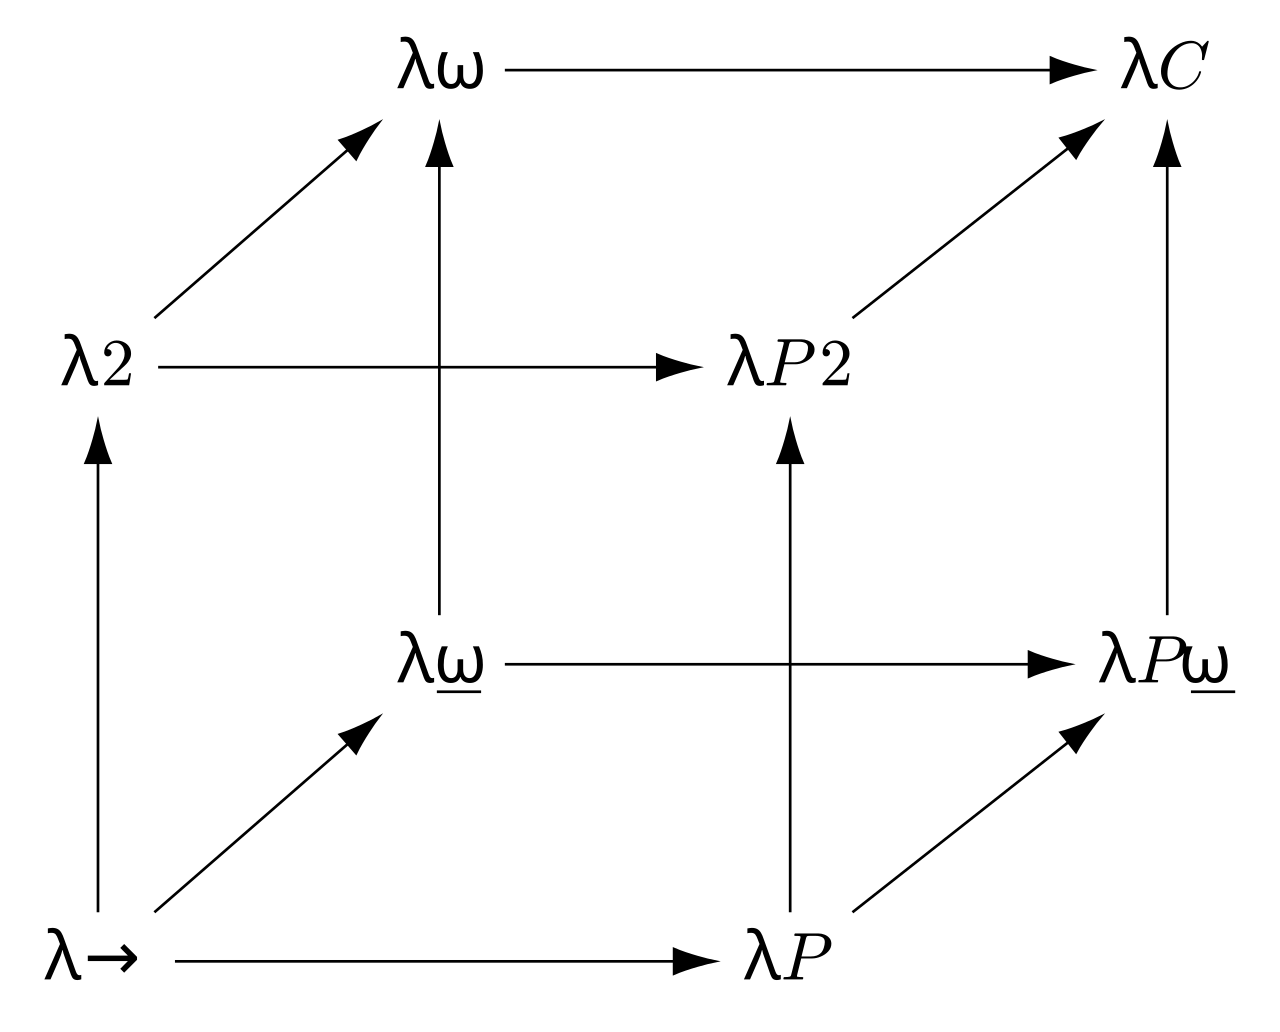
\includegraphics[width=0.7\columnwidth]{lambda_cube.png}
    \caption{مکعب لامبدا}
    \label{fig:lambda-cube}
\end{figure}

حال با معرفی کامل سیستم‌های نوع محض، بسیاری از سیستم‌های مشهور تنها با انتخاب مناسب
$(\mathcal{S},\mathcal{A},\mathcal{R})$
قابل بیان‌اند. همان‌طور که در جدول \ref{tab:lambda-cube} مشاهده می‌شود، هر هشت راس مکعب لامبدا را می‌توان به کمک سیستم‌های نوع محض تعریف کرد.

\begin{table}[ht]
\centering
\caption{بیان مکعب لامبدا به کمک سیستم‌های نوع محض}
\label{tab:lambda-cube}
\renewcommand{\arraystretch}{1.5}
\resizebox{\columnwidth}{!}{%
\begin{tabular}{c|c|c|c}
$\mathcal{R}$ & $\mathcal{A}$ & $\mathcal{S}$ & سیستم نوع \\
\hline\hline
$\{(*,*,*)\}$ & $\{(*,\Box)\}$ & $\{*,\Box\}$ & $\lambda \to$ \\
$\{(*,*,*),(\Box,*,*)\}$ & $\{(*,\Box)\}$ & $\{*,\Box\}$ & $\lambda 2$ \\
$\{(*,*,*),(\Box,\Box,\Box)\}$ & $\{(*,\Box)\}$ & $\{*,\Box\}$ & $\lambda \underline{\omega}$ \\
$\{(*,*,*),(*,\Box,\Box)\}$ & $\{(*,\Box)\}$ & $\{*,\Box\}$ & $\lambda P$ \\
$\{(*,*,*),(*,\Box,\Box),(\Box,*,*)\}$ & $\{(*,\Box)\}$ & $\{*,\Box\}$ & $\lambda P2$ \\
$\{(*,*,*),(\Box,\Box,\Box),(\Box,*,*)\}$ & $\{(*,\Box)\}$ & $\{*,\Box\}$ & $\lambda \omega$ \\
$\{(*,*,*),(\Box,\Box,\Box),(*,\Box,\Box)\}$ & $\{(*,\Box)\}$ & $\{*,\Box\}$ & $\lambda P\underline{\omega}$ \\
$\{(*,*,*),(\Box,\Box,\Box),(*,\Box,\Box),(\Box,*,*)\}$ & $\{(*,\Box)\}$ & $\{*,\Box\}$ & $\lambda C$
\end{tabular}%
}
\end{table}

\subsection{سیستم‌های نوع محض لایه‌ای}

\begin{definition}\label{tpts_signature}
یک سیستم نوع محض، \lr{n}-لایه‌ای است، هرگاه مشخصه آن به فرم زیر باشد:
\vspace{-5pt}
\begin{align*}
\mathcal{S} &= \{ s_i \mid i \in \{1,\dots,n\} \}\\
\mathcal{A} &= \{ (s_i,s_{i+1}) \mid i \in \{1,\dots,n{-}1\} \}\\
\mathcal{R} &\subset \{ (s,s',s') \mid (s,s') \in \mathcal{S} \times \mathcal{S} \}
\end{align*}
\end{definition}

\begin{remark}
\hfil
\begin{itemize}[noitemsep, topsep=0pt]
  \item[-] سیستم نوع محض صفر-لایه‌ای $\equiv$ سیستم نوع محض تهی ($\mathcal{S}=\mathcal{A}=\mathcal{R}=\emptyset$)
  \item[-] سیستم‌های نوع محض ۲-لایه‌ای که شامل قانون $(s_1, s_1, s_1)$ هستند $\equiv$ کل مکعب لامبدا
\end{itemize}
\end{remark}

\begin{definition}
درجه هر عبارت در سیستم‌های نوع محض لایه‌ای، با تابع $\operatorname{deg}: \mathrm{T} \to \mathbb{N}$ به صورت زیر محاسبه می‌شود:
\vspace{-5pt}
\begin{align*}
\operatorname{deg}(s_i) &= i + 1\\
\operatorname{deg}(^{s_i}x) &= i - 1\\
\operatorname{deg}(\Pi x^A.B) &= \operatorname{deg}(B)\\
\operatorname{deg}(\lambda x^A.M) &= \operatorname{deg}(M)\\
\operatorname{deg}(MN) &= \operatorname{deg}(M)
\end{align*}
همچنین می‌نویسیم:
\vspace{-5pt}
\begin{align*}
\mathrm{T}_j &= \{M \in \mathrm{T} \mid \operatorname{deg}(M) = j\}\\
\mathrm{T}_{\ge j} &= \{M \in \mathrm{T} \mid \operatorname{deg}(M) \ge j\}
\end{align*}
\end{definition}

\begin{definition}
یک سیستم نوع محض لایه‌ای،
$(i,j)$-کامل \LTRfootnote{$(i,j)-\text{\lr{full}}$}
است، اگر قوانین آن شامل
\vspace{-5pt}
\begin{equation*}
\{(s_l,s_k) \mid (l \le i) \land (l \le k \le j)\}
\end{equation*}
باشد؛ و کامل است، هرگاه به ازای هر
$(s_i,s_j) \in \mathcal{R}$،
این سیستم
$(j,i)$-کامل باشد.
\end{definition}

\subsection{ترجمه حذف وابستگی}

\begin{definition}\label{non_dependent}
نسخه غیروابسته یک سیستم نوع محض لایه‌ای
$\lambda S$،
که با
$\lambda S^*$
نشان داده می‌شود، سیستمی با مشخصه زیر است:
\vspace{-5pt}
\begin{align*}
S_{\lambda S^*} &= S_{\lambda S}\\
\mathcal{A}_{\lambda S^*} &= \mathcal{A}_{\lambda S}\\
\mathcal{R}_{\lambda S^*} &= \{(s_i,s_j,s_j) \in \mathcal{R}_{\lambda S} \mid (i \ge j)\}
\end{align*}
\end{definition}

می‌خواهیم یک ترجمه از سیستم نوع محض لایه‌ای
$\lambda S$
به نسخه غیروابسته آن، یعنی
$\lambda S^*$
ارائه کنیم، به طوری که خواص حفظ نوع و حفظ مسیرهای کاهش نامتناهی را دارا باشد. الزامات روی ساختار غیروابسته کاملاً قوی خواهند بود.

\begin{definition}[ترجمه سطح نوع\LTRfootnote{Type-Level Translation}]\label{rho_def}
\hfil{}\\
برای هر
$0 \le i \le n$،
تابع
$\rho_i : \mathrm{T}_{\ge i+1} \to \mathrm{T}_{i+1}$
به صورت استقرایی زیر تعریف می‌شود:
\vspace{-5pt}
\begin{align*}
\rho_i(s_j) &= 
    \begin{cases}
        0 &i = 0\\
        s_i &\text{\lr{o.w}}
    \end{cases}\\
\rho_i({}^{s_j}x) &= {}^{s_{i+2}}x \quad (j \ge i+2)\\
\rho_i(\Pi x^A.B) &= \Pi x^{\rho_{\operatorname{deg} A-1}(A)} \dots \Pi x^{\rho_{i}(A)}.\rho_i(B)\\
\rho_i(\lambda x^A.M) &= \lambda x^{\rho_{\operatorname{deg} A-1}(A)} \dots \lambda x^{\rho_{i+1}(A)}.\rho_i(M)\\
\rho_i(MN) &= \rho_i(M) \rho_{\operatorname{deg} N-1}(N) \dots \rho_i(N)
\end{align*}
که در آن
\lr{0}
یک متغیر منحصر به فرد است.

تعریف هر ترجمه محدود به مواردی است که برای آن‌ها عباراتی در دامنه مورد نظر وجود دارد. برای مثال، پایه‌ای‌ترین ترجمه
$\rho_n : \mathrm{T}_{\ge n+1} \to \mathrm{T}_{n+1}$
فقط بر روی
$\{s_n\}$
با ضابطه
$\rho_n(s_n) = s_n$
تعریف می‌شود و بقیه حالات نادیده گرفته می‌شوند. این ترجمه‌ها به زمینه‌ها نیز به شرح زیر گسترش می‌یابند:
\vspace{-5pt}
\resizedalign{
\rho_i(\varnothing) &= (0 : s_1)\\
\rho_i(\Gamma,{}^{s_{j}}x:A) &= \rho_i(\Gamma),{}^{s_{j}}x:\rho_{j-1}(A),\dots,{}^{s_{i+1}}x:\rho_{i}(A) \quad{\scriptstyle (j \ge i+1)}
}
\end{definition}

\begin{lemma}
برای هر
$0 \le i \le n$
و هر
$1 \le j \le n$
و هر عبارت
$A$ و $B$،
اگر
$A \in \mathrm{T}_{\ge i+1}$ و $\operatorname{deg} B = j-1$، آنگاه
\vspace{-5pt}
\resizedalign{
\rho_i(A[B/{}^{s_j}x]) = \rho_i(A)[\rho_{j-2}(B)/{}^{s_j}x] \dots [\rho_{i}(B)/{}^{s_{i+2}}x]
}
\end{lemma}

\begin{lemma}
برای هر
$0 \le i \le n$
و هر عبارت
$A$ و $B$،
اگر
$A \in \mathrm{T}_{\ge i+1}$ و $A \twoheadrightarrow_\beta B$، آنگاه
\vspace{-5pt}
\begin{equation*}
\rho_i(A) \twoheadrightarrow_\beta \rho_i(B)
\end{equation*}
\end{lemma}

\begin{lemma}
برای هر
$0 \le i \le n$،
اگر
$\Gamma$ یک زمینه و
$A$ و $B$ عباراتی باشند که
$A \in \mathrm{T}_{\ge i+1}$ و $\Gamma \vdash_{\lambda S} A : B$، آنگاه
\vspace{-5pt}
\begin{equation*}
\rho_{i+1}(\Gamma) \vdash_{\lambda S^*} \rho_i(A) : \rho_{i+1}(B)
\end{equation*}
\end{lemma}

\begin{definition}[ترجمه سطح عبارت\LTRfootnote{Term-Level Translation}]\label{gamma_def}
تابع
$\gamma : \mathrm{T} \to \mathrm{T}$
به صورت استقرایی زیر تعریف می‌شود:
\vspace{-5pt}
\[
\resizebox{\columnwidth}{!}{$
\begin{aligned}
\gamma(s_i) &= \bullet\\
\gamma({}^{s_i}x) &= {}^{s_1}x\\
\gamma(\Pi x^A.B) &= \operatorname{prod}(\Pi x^{\rho_{deg A - 1}(A)} \dots \Pi x^{\rho_{0}(A)}.0) \\ &\gamma(A) (\lambda x^{\rho_{deg A - 1}(A)} \dots \lambda x^{\rho_{0}(A)}.\gamma(B))\\
\gamma(\lambda x^A.M) &= (\lambda z^0.\lambda x^{\rho_{deg A - 1}(A)} \dots \lambda x^{\rho_{0}(A)}.\gamma(M)) \gamma(A)\\
\gamma(MN) &= \gamma(M) \rho_{degN-1}(N) \dots \rho_{0}(N) \gamma(N)
\end{aligned}
$}
\]
که در آن
$\{\operatorname{prod}, \bullet, z\}$
متغیرهای منحصر به فردی هستند.
\end{definition}

سه لمی که در بخش قبل بررسی کردیم، برای ترجمه سطح عبارت نیز قابل بیان هستند.

\begin{lemma}\label{preserve_type}
برای هر عبارت
$A$ و $B$،
اگر $\Gamma \vdash_{\lambda S} A:B$، آنگاه
\vspace{-5pt}
\begin{align*}
\Delta \; := \; 0 : s_1,\; \bullet : 0,\; &\operatorname{prod} : \Pi A^{s_1}.0 \to A \to 0\\
\Delta, \; \rho_0(\Gamma) \; &\vdash_{\lambda S^*} \; \gamma(A) : \rho_0(B)
\end{align*}
\end{lemma}

\begin{lemma}
برای هر
$1 \le j \le n$،
و هر عبارت
$A$ و $B$ که $\operatorname{deg}(B) = j-1$، داریم:
\vspace{-5pt}
\resizedalign{
\gamma(A[B/{}^{s_{j}}x]) = \gamma(A) [\rho_{j-2}(B)/{}^{s_{j}}x] \dots [\rho_{0}(B)/{}^{s_{2}}x] [\gamma(B)/{}^{s_{1}}x]
}
\end{lemma}

\begin{lemma}\label{preserve_reduction}
برای هر عبارت
$A$ و $B$، اگر $A \to_\beta B$، آنگاه
\vspace{-5pt}
\begin{equation*}
\gamma(A) \twoheadrightarrow^+_\beta \gamma(B)
\end{equation*}
\end{lemma}

\begin{theorem}\label{main_theorem}
فرض کنید
$\lambda S$
یک سیستم نوع محض
$n$-لایه‌ای
است که تا یک مقدار
$i$
کامل است ($i<n$).
$\lambda S$ دارای خاصیت نرمال‌سازی قوی است، اگر و تنها اگر $\lambda S^*$ چنین باشد.
\end{theorem}

\begin{proof}
از آنجایی که همه عبارات قابل استنتاج
$\lambda S^*$، در $\lambda S$ نیز استنتاج می‌شوند،
اگر $\lambda S$ دارای خاصیت نرمال‌سازی قوی باشد آنگاه $\lambda S^*$ نیز دارای این خاصیت خواهد بود.\\
حال فرض کنید
$\lambda S$ دارای خاصیت نرمال‌سازی قوی نباشد. پس یک دنباله کاهش نامتناهی مانند
\vspace{-5pt}
\begin{equation*}
M_1 \to_\beta M_2 \to_\beta \dots
\end{equation*}
در آن وجود دارد.
طبق لم‌های \ref{preserve_type} و \ref{preserve_reduction}، می‌توان گفت دنباله کاهش نامتناهی
\vspace{-5pt}
\begin{equation*}
\gamma(M_1) \twoheadrightarrow^+_\beta \gamma(M_2) \twoheadrightarrow^+_\beta \dots
\end{equation*}
در
$\lambda S^*$
یافت می‌شود، که با فرض آنکه
$\lambda S^*$
دارای خاصیت نرمال‌سازی قوی است، در تناقض است.
\end{proof}

تنها سیستم جالب‌توجهی که این قضیه بر آن قابل اعمال است، سیستم
$n$-لایه‌ای
با قوانین زیر است:
\vspace{-5pt}
\resizedalign{
\{(s_k,s_1) \mid k \in [n]\} \cup \{(s_1,s_k) \mid k \in [n]\} \cup \{(s_2,s_k) \mid k \in [n]\}    
}
و همچنین هر زیرسیستمی از آن که دارای همین قوانین غیروابسته باشد.
قضیه
\ref{main_theorem}
بیان می‌کند که خاصیت نرمال‌سازی قوی برای این سیستم، معادل همین خاصیت برای سیستم با قوانین زیر است:
\vspace{-5pt}
\begin{equation*}
\{(s_k,s_1) \mid k \in [n]\} \cup \{(s_2,s_2)\}
\end{equation*}
هرچند می‌توان این نتیجه را به‌صورت صوری نیز اثبات کرد، بررسی اجمالی این روش نشان می‌دهد که از دیدگاه فرا‌نظری، این روش ضعیف است و می‌توان آن را در حساب پئانو \LTRfootnote{Peano Arithmetic} اجرا کرد.
از این‌ رو، با ترکیب این نتیجه با نتیجه‌ی
\cite{barthe2001}،
به حالت خاصی از حدس
\lr{BGK}
دست می‌یابیم.

\begin{corollary}\label{cor}
در سیستم نوع محض
$n$-لایه‌ای
با قوانین
\vspace{-5pt}
\resizedalign{
\{(s_k,s_1) \mid k \in [n]\} \cup \{(s_1,s_k) \mid k \in [n]\} \cup \{(s_2,s_k) \mid k \in [n]\}    
}
نرمال‌سازی ضعیف مستلزم نرمال‌سازی قوی است. همچنین، این اثبات را می‌توان در حساب پئانو انجام داد.
\end{corollary}

\begin{definition}
اصول موضوعه پئانو، اعداد طبیعی را به صورت زیر مشخص می‌کند:
\begin{itemize}[noitemsep, topsep=0pt]
    \item[-] صفر یک عدد طبیعی است.
    \item[-] اگر $a$ یک عدد طبیعی باشد، تالی آن ($S(a)$) نیز عددی طبیعی است.
    \item[-] اگر تالی دو عدد طبیعی برابر باشد، خود آن اعداد نیز با هم برابرند.
    \item[-] (اصل استقرا): اگر مجموعه اعداد $\mathrm{S}$ شامل صفر و تالی هر عدد موجود در $\mathrm{S}$ باشد، آنگاه همه اعداد در $\mathrm{S}$ هستند.
\end{itemize}
\end{definition}

\section{$\overline{\text{
صوری‌سازی
}}$}

فایل‌های صوری‌سازی در \cite{thesis-code} در دسترس هستند. در این بخش به توضیح نکات و تصمیمات اتخاذ شده می‌پردازیم. مطالعه کد اصلی در کنار این بخش، مفید خواهد بود.

\subsection{رویکرد و معماری}

در این پژوهش، به‌منظور صوری‌سازی تعاریف و نتایج مربوط به ترجمه حذف وابستگی در سیستم‌های نوع محض لایه‌ای، از اثبات‌یار
\lr{Rocq} \LTRfootnote{The Rocq Prover, version 9.2}
استفاده شده است. رویکرد اتخاذشده مبتنی بر تفکیک مشخصات سیستم‌های نوع از تعاریف و اثبات‌های مربوط به آن‌ها است. به این منظور، از سازوکار ماژول‌ها \LTRfootnote{Modules} در
\lr{Rocq}
استفاده شده تا مشخصات هر سیستم نوع به‌صورت مستقل تعریف شده و تعاریف و قضایای متناظر با آن به‌صورت پارامتری توسعه یابند.

ساختار پیاده‌سازی از چهار فایل اصلی تشکیل شده است که در دو گروه مشخصات و صوری‌سازی سازمان‌دهی شده‌اند.
فایل‌های \filename{PTSSignature.v} و \filename{TPTSSignature.v}
مشخصات سیستم‌های نوع محض و سیستم‌های نوع محض لایه‌ای را تعریف می‌کنند. در مقابل، فایل‌های \filename{PTS.v} و \filename{TPTS.v}
شامل تعاریف صوری، لم‌ها و اثبات‌های مربوط به این ساختارها هستند.

در فایل \filename{PTSSignature.v}،
مشخصه عمومی یک سیستم نوع محض با استفاده از یک نوع ماژولی \LTRfootnote{Module Type} تعریف شده است.
به این ترتیب، مشخصات یک سیستم نوع محض بدون وابستگی به نمونه مشخصی از آن بیان می‌شود.
سپس در فایل \filename{PTS.v}،
با دریافت یک نمونه از مشخصه مذکور به‌عنوان پارامتر ورودی، تعاریف و لم‌های عمومی سیستم نوع محض توسعه داده شده‌اند. استفاده از این ساختار پارامتری موجب می‌شود که نتایج صوری‌سازی‌شده مستقل از انتخاب یک سیستم نوع محض خاص باشند و برای هر نمونه سازگار با مشخصه تعریف‌شده قابل استفاده باشند.

در مرحله بعد، به‌منظور مدل‌سازی سیستم‌های نوع محض لایه‌ای، مشخصه جدیدی در فایل
\filename{TPTSSignature.v}
تعریف شده است. این مشخصه با استفاده از مشخصه سیستم نوع محض توسعه یافته و علاوه بر ساختارهای پایه، شامل پارامترها و قیود مربوط به سیستم‌های نوع محض لایه‌ای است.
این مشخصات، شرایط صوری لازم برای مدل‌سازی سیستم نوع محض لایه‌ای را فراهم می‌کنند.
در نهایت، فایل \filename{TPTS.v} به صوری‌سازی سیستم نوع محض لایه‌ای اختصاص یافته است.
در این فایل، علاوه بر دریافت مشخصه سیستم نوع محض لایه‌ای، از ماژول صوری‌سازی‌شده سیستم نوع محض،
یعنی \filename{PTS.v}،
استفاده مجدد شده است. بدین منظور، یک نمونه از ماژول
\filename{PTS}
بر اساس مشخصه ورودی ساخته شده و تعاریف و لم‌های آن در توسعه ساختار لایه‌ای مورد استفاده قرار گرفته‌اند. پس از آن، تعاریف مربوط به ترجمه حذف وابستگی، لم‌های موردنیاز و قضایای مرتبط با صحت این ترجمه صوری‌سازی و اثبات شده‌اند.

این معماری با تفکیک مشخصات از پیاده‌سازی و استفاده مجدد از تعاریف و نتایج عمومی، از تکرار بخش‌های مشترک میان دو سیستم جلوگیری کرده و امکان سازمان‌دهی مستقل و توسعه‌پذیر اثبات‌ها را فراهم می‌کند. ساختار وابستگی میان فایل‌های پروژه در شکل (۱) نشان داده شده است.

\begin{figure}[ht]
    \centering
    \begin{tikzpicture}[
        scale=0.75,
        transform shape,
        file/.style={
            draw,
            rounded corners=2pt,
            minimum width=3.2cm,
            minimum height=0.8cm,
            align=center,
            font=\small
        },
        dependency/.style={
            -{Stealth},
            thick
        }
    ]

    \node[file] (sig) {
        \filename{PTSSignature.v}
    };

    \node[file, below left=1.3cm and 0.3cm of sig] (pts) {
        \filename{PTS.v}
    };

    \node[file, below right=1.3cm and 0.3cm of sig] (tptssig) {
        \filename{TPTSSignature.v}
    };

    \node[file, below=2.6cm of sig] (tpts) {
        \filename{TPTS.v}
    };

    \draw[dependency] (sig) -- (pts);
    \draw[dependency] (sig) -- (tptssig);
    \draw[dependency] (pts) -- (tpts);
    \draw[dependency] (tptssig) -- (tpts);

    \end{tikzpicture}
    \caption{ساختار وابستگی فایل‌های صوری‌سازی}
    \label{fig:formalization-architecture}
\end{figure}

\subsection{صوری‌سازی مشخصه سیستم‌ها}

به‌منظور صوری‌سازی مشخصه سیستم نوع محض معرفی‌شده در تعریف \ref{pts_signature}، از سازوکار نوع‌های ماژولی استفاده شده است:

\begin{latin}
\begin{lstlisting}[
    style=Rocqstyle,
    label={lst:pts-signature}
]
(* Source: PTSSignature.v *)
Module Type PTS_SIGNATURE.
  Parameter Sort : Type.
  Parameter A : Sort -> Sort -> Prop.
  Parameter R : Sort -> Sort -> Sort -> Prop.
End PTS_SIGNATURE.
\end{lstlisting}
\end{latin}

در این مشخصه پارامتر \varname{Sort} مجموعه رده‌های سیستم را مشخص می‌کند. همچنین رابطه دوتایی \varname{A} و رابطه سه‌تایی \varname{R} به ترتیب متناظر با روابط $\mathcal{A}$ و $\mathcal{R}$ در تعریف ریاضی سیستم نوع محض هستند. استفاده از نوع \varname{Prop} برای این دو پارامتر بیانگر آن است که این مولفه‌ها به صورت گزاره‌ای و رابطه‌ای تعریف شده‌اند.

استفاده از \varname{Module Type} امکان تعریف مشخصه سیستم نوع محض را بدون تعیین یک نمونه مشخص از آن فراهم می‌کند. در نتیجه، ماژول‌های بعدی می‌توانند با دریافت یک نمونه سازگار با این مشخصه، تعاریف و نتایج عمومی مربوط به سیستم نوع محض را توسعه دهند.

به طور مشابه، به‌منظور صوری‌سازی مشخصه سیستم نوع محض لایه‌ای معرفی‌شده در تعریف \ref{tpts_signature}، از سازوکار نوع‌های ماژولی استفاده شده است:

\begin{latin}
\begin{lstlisting}[
    style=Rocqstyle,
    label={lst:tpts-signature}
]
(* Source: TPTSSignature.v *)
Module Type TPTS_SIGNATURE <: PTS_SIGNATURE.
  Include PTS_SIGNATURE.
  Parameter n : nat.
  Parameter index_of : Sort -> nat.
  Axiom n_range : n > 0.
  Axiom index_range : forall x, 
    0 < index_of x /\ index_of x < n + 1.
  Axiom index_inj : forall x y, 
    index_of x = index_of y -> x = y.
  Axiom index_surj : forall i : nat, 
    0 < i /\ i < n + 1 -> 
    exists x : Sort, index_of x = i.
  Axiom A_spec : forall x y, 
    A x y <-> index_of x < n /\ 
              index_of y = S (index_of x).
  Axiom R_shape : forall x y z, 
    R x y z -> y = z.
End TPTS_SIGNATURE.
\end{lstlisting}
\end{latin}

این مشخصه، از مشخصه سیستم نوع محض ارث‌بری می‌کند و به این معناست که نمونه‌ای از مشخصه سیستم‌های نوع محض است. به منظور پیاده‌سازی مشخصه یک سیستم نوع محض لایه‌ای، نیاز به دو پارامتر جدید داریم؛ پارامتر \varname{n} که بیانگر تعداد لایه‌های سیستم است و پارامتر \varname{index_of} که نحوه اندیس‌گذاری رده‌ها را معین می‌کند. مقادیر این دو پارامتر جدید، توسط قیودی مدیریت می‌شوند:
\begin{itemize}[noitemsep, topsep=0pt]
    \item[-] \varname{n_range}: تعداد لایه‌ها باید بیشتر از صفر باشد.
    \item[-] \varname{index_range}: اندیس هر رده، حداقل ۱ و حداکثر \varname{n} است.
    \item[-] \varname{index_inj}: تابع اندیس‌گذار، یک‌به‌یک است.
    \item[-] \varname{index_surj}: تابع اندیس‌گذار، پوشاست.
\end{itemize}

حال که توانستیم اندیس‌گذاری را به مشخصه اضافه کنیم، با دو قید دیگر، مشخصه سیستم مدنظر \lr{Mull} را تکمیل می‌کنیم. قید \varname{A_spec} بیانگر آن است که رابطه $\mathcal{A}$ بین اندیس‌های متوالی برقرار است و قید \varname{R_shape} به معنای یکسان بودن رده دوم و سوم در رابطه $\mathcal{R}$ است.

\subsection{صوری‌سازی سیستم‌های نوع محض}

پس از تعریف مشخصه سیستم نوع محض، در گام بعدی ساختار عمومی این سیستم در قالب یک ماژول تعریف می‌شود:
\begin{latin}
\begin{lstlisting}[
    style=Rocqstyle,
    label={lst:pts}
]
(* Source: PTS.v *)
Module PTS (Sig : PTS_SIGNATURE).
Import Sig.
\end{lstlisting}
\end{latin}

ماژول \varname{PTS} با دریافت یک پارامتر از نوع \varname{PTS_SIGNATURE} تعریف شده است و سپس با استفاده از \varname{Import Sig}، مؤلفه‌های معرفی‌شده در این مشخصه، از جمله مجموعه رده‌ها و روابط مربوط به آن، درون ماژول در دسترس قرار می‌گیرند. به این ترتیب، تعریف سیستم نوع محض مستقل از یک نمونه خاص از مشخصه آن انجام می‌شود و امکان استفاده مجدد از این تعریف برای سیستم‌های مختلفی که با مشخصه مذکور سازگارند، فراهم می‌شود.

برای بازنمایی نحو عبارات و مدیریت متغیرهای مقید، از روش بی‌نام محلی استفاده شده است. در این روش، متغیرهای آزاد با استفاده از نام یا شناسه مشخص و متغیرهای مقید با استفاده از اندیس‌های دبروین\LTRfootnote{de Bruijn indices} نمایش داده می‌شوند. به این ترتیب، تغییر نام متغیرهای مقید تأثیری بر نمایش صوری عبارت نخواهد داشت. در نتیجه، مسائلی مانند تغییر نام متغیرهای مقید و برخورد نام متغیرها \LTRfootnote{Variable Capture} ساده‌تر مدیریت می‌شوند. مطابق این روش، در تعریف نوع استقرایی \varname{term}، سازنده‌های \varname{t_bvar} و \varname{t_fvar} به ترتیب برای نمایش متغیرهای مقید و آزاد در نظر گرفته شده اند:
\begin{latin}
\begin{lstlisting}[
    style=Rocqstyle,
    label={lst:term}
]
(* Source: PTS.v *)
Inductive term : Type :=
  | t_sort : Sort -> term
  | t_bvar : Sort -> nat -> term
  | t_fvar : Sort -> var -> term
  | t_app  : term -> term -> term
  | t_lam  : Sort -> term -> term -> term
  | t_pi   : Sort -> term -> term -> term.
\end{lstlisting}
\end{latin}

در این تعریف، شناسه متغیرها با استفاده از اعداد طبیعی نمایش داده می‌شود و رده هر رخداد متغیر، اعم از آزاد یا مقید، به‌صورت برچسبی صریح در ساختار آن ذخیره می‌شود. همچنین، مقیدکننده‌ها (\varname{t_lam} و \varname{t_pi}) رده دامنه خود را نگهداری می‌کنند. این برچسب‌گذاری، متناظر با ملاحظه \ref{sort_tag} انجام شده و اطلاعات لازم برای محاسبه درجه عبارت را فراهم می‌کند.

انتخاب روش بی‌نام محلی برای صوری‌سازی متغیرها، آورده‌های فراوانی در ادامه کار داشته است. یکی از مهم‌ترین آن‌ها، تعریف جانشینی است که به دلیل آن که نگران برخورد متغیرها نیستیم، بسیار ساده‌تر از تعریف \ref{subst} نوشته می‌شود:

\begin{latin}
\begin{lstlisting}[
    style=Rocqstyle,
    label={lst:term}
]
(* Source: PTS.v *)
Fixpoint subst_term (x : var) (N : term) 
                    (t : term) : term :=
  match t with
  | t_sort s => t_sort s
  | t_bvar s n => t_bvar s n
  | t_fvar s y => if eq_var_dec y x then N else t_fvar s y
  | t_app P Q => t_app P[x := N] Q[x := N]
  | t_pi s A B => t_pi s A[x := N] B[x := N]
  | t_lam s A M => t_lam s A[x := N] M[x := N]
  end
\end{lstlisting}
\end{latin}

حال که از روش بی‌نام محلی استفاده کرده‌ایم و متغیرها و دامنه عبارات $\lambda$ و $\Pi$ را با رده‌ برچسب‌گذاری کرده‌ایم، قاعده تشکیل نوع تابع از مجموعه قواعد استنتاج نوع، ارزش بررسی به‌خصوصی دارد:
\begin{latin}
\begin{lstlisting}[
    style=Rocqstyle,
    label={lst:term}
]
(* Source: PTS.v *)
Inductive typing : 
  context -> term -> term -> Prop :=
  ...
  | typing_pi : forall C A B s1 s2 s3 L,
      C |- A : t_sort s1 ->
      bvar_tag_ok 0 s1 B ->
      (forall x, ~ In x L ->
         C ++ [(x, (s1, A))] |- 
          (open_var B s1 x) : t_sort s2) ->
      R s1 s2 s3 ->
      C |- (t_pi s1 A B) : (t_sort s3)
  
\end{lstlisting}
\end{latin}

تفاوت‌هایی که با تعریف \ref{typing} مشهود است:
\begin{itemize}[noitemsep, topsep=0pt]
  \item[-] در اینجا نیاز به بررسی سازگاری رده برچسب‌گذاری شده و رده عبارت \varname{B} داریم. شرط \varname{bvar_tag_ok 0 s1 B} این مورد را تضمین می‌کند.
  \item[-] برای جلوگیری از وابستگی قاعده به نام مشخصی برای متغیر مقید، از مجموعه متناهی \varname{L} استفاده شده است. این مجموعه شامل نام‌هایی است که نباید برای بازکردن متغیر مقید انتخاب شوند. بنابراین، شرط نوع‌گذاری بدنه برای هر متغیر خارج از \varname{L} بررسی می‌شود. این سازوکار امکان انتخاب نام تازه برای متغیر مقید را فراهم کرده و با رویکرد نمایش بی‌نام محلی سازگار است.
\end{itemize}

\subsection{صوری‌سازی سیستم‌های نوع محض لایه‌ای}

مشابه سیستم‌ نوع محض، سیستم نوع محض لایه‌ای نیز در قالب یک ماژول تعریف می‌شود:
\begin{latin}
\begin{lstlisting}[
    style=Rocqstyle,
    label={lst:tpts}
]
(* Source: TPTS.v *)
Module TPTS (Sig : TPTS_SIGNATURE).
Import Sig.
Module Base := PTS Sig.
Import Base.
\end{lstlisting}
\end{latin}

در این قسمت، ابتدا مؤلفه‌های مشخصه سیستم نوع محض لایه‌ای در دسترس ماژول قرار می‌گیرند. سپس، با استفاده از دستور \varname{Module Base := PTS Sig}، نمونه‌ای از ماژول عمومی سیستم نوع محض با دریافت مشخصه \varname{Sig} ایجاد می‌شود. این نمونه شامل تعاریف و نتایج صوری‌سازی‌شده مربوط به سیستم نوع محض است که با استفاده از دستور \varname{Import Base} در ادامه پیاده‌سازی سیستم نوع محض لایه‌ای قابل استفاده خواهند بود. به این ترتیب، از آنجا که سیستم نوع محض لایه‌ای، ساختار پایه یک سیستم نوع محض را نیز داراست، تعاریف و نتایج مربوط به سیستم پایه بدون نیاز به بازتعریف در صوری‌سازی \varname{TPTS} مورد استفاده قرار می‌گیرند.

برچسب‌گذاری متغیرها با رده، در تعریف تابع درجه استفاده می‌شود:
\begin{latin}
\begin{lstlisting}[
    style=Rocqstyle,
    label={lst:tpts}
]
(* Source: TPTS.v *)
Fixpoint deg (t : term) : nat :=
  match t with
  | t_sort s     => index_of s + 1
  | t_bvar s _   => index_of s - 1
  | t_fvar s _   => index_of s - 1
  | t_app M _    => deg M
  | t_lam _ _ M  => deg M
  | t_pi  _ _ B  => deg B
  end.
\end{lstlisting}
\end{latin}

برای ادامه کار، \lr{Mull} یک سیستم نوع محض لایه‌ای کامل را، ثابت فرض می‌کند. ما نیز این فرض را صوری‌سازی می‌کنیم (\varname{is_full}):
\begin{latin}
\begin{lstlisting}[
    style=Rocqstyle,
    label={lst:full}
]
(* Source: TPTS.v *)
Definition full_with (i j : nat) : Prop :=
  forall l k : Sort, index_of l <= i ->
  index_of l <= index_of k -> 
  index_of k <= j -> R l k k.
Definition full : Prop :=
  forall s1 s2 s3, R s1 s2 s3 -> 
  full_with (index_of s2) (index_of s1).
Axiom is_full : full.
\end{lstlisting}
\end{latin}

همانطور که در تعریف \ref{non_dependent} دیدیم، نسخه غیروابسته یک سیستم نوع محض لایه‌ای، فقط در مجموعه $\mathcal{R}$ با آن متفاوت است. به منظور صوری‌سازی این نسخه، باید توجه کنیم که مجموعه مذکور صرفا در قاعده تشکیل نوع تابع، از مجموعه قواعد استنتاج نوع در تعریف \ref{typing}، کاربرد دارد؛ بنابراین کافی است قواعد استنتاج نوع را به کمک $\mathcal{R}^*$ بازتعریف کنیم تا نسخه غیروابسته یک سیستم نوع محض لایه‌ای، صوری‌سازی شود:
\begin{latin}
\begin{lstlisting}[
    style=Rocqstyle,
    label={lst:typing-star}
]
(* Source: TPTS.v *)
Definition R_star (s s' s'' : Sort) : Prop :=
  R s s' s'' /\ index_of s' <= index_of s.

Inductive typing_star : 
  context -> term -> term -> Prop :=
  ...
  | typing_star_pi : forall C A B s1 s2 s3 L,
      C |-* A : t_sort s1 ->
      ... ->
      R_star s1 s2 s3 ->
      C |-* (t_pi s1 A B) : (t_sort s3)
\end{lstlisting}
\end{latin}

حال با توجه به آنکه دو مجموعه قواعد استنتاج نوع داریم (اصلی و غیروابسته)، نیاز به دو محمول مجزا برای نوع‌پذیری داریم:
\begin{latin}
\begin{lstlisting}[
    style=Rocqstyle,
    label={lst:derivable}
]
(* Source: TPTS.v *)
Definition derivable (M : term) : Prop := 
  exists C N, C |- M : N.
Definition derivable_star (M : term) : Prop :=
  exists C N, C |-* M : N.
\end{lstlisting}
\end{latin}
اکنون خاصیت نرمال‌سازی قوی سیستم را طوری تعریف می‌کنیم که محمول نوع‌پذیری را در ورودی بپذیرد:
\begin{latin}
\begin{lstlisting}[
    style=Rocqstyle,
    label={lst:sn}
]
(* Source: TPTS.v *)
Definition system_strongly_normalizing 
  (P : term -> Prop) : Prop :=
  forall M, P M -> strongly_normalizing M.
\end{lstlisting}
\end{latin}

در ادامه به تابع ترجمه سطح نوع با نام \varname{rho} می‌پردازیم. این تابع را به صورت بازگشتی بر حسب ساختار عبارت ورودی تعریف می‌کنیم. به تعریف این تابع در حالتی که ورودی یک عبارت $\Pi$ است دقت کنید:
\begin{latin}
\begin{lstlisting}[
    style=Rocqstyle,
    label={lst:rho}
]
(* Source: TPTS.v *)
Fixpoint rho (i : nat) (M : term) : term :=
  match M with
  ...
  | t_pi s A B =>
      match le_lt_dec (i + 1) (deg A) with
      | left _  => 
        rho_pi_tel rho A B i (deg A - 1 - i)
      | right _ => 
        rho i B
      end
  ...
  end.
\end{lstlisting}
\end{latin}
مطابق تعریف \ref{rho_def}، خروجی در این حالت یک زنجیره از عبارت $\Pi$ است. ایده پیاده‌سازی چنین است که ابتدا وجود این زنجیره را بررسی می‌کنیم؛ اگر $\operatorname{deg}A \ge i + 1$ باشد، زنجیره به کمک تابع \varname{rho_pi_tel} تشکیل می‌شود، در غیر این صورت زنجیره تشکیل نشده و فقط $\rho_i(B)$ در خروجی باقی می‌ماند. این ایده از روشی که \lr{Mull} در اثبات لم‌های مربوط به این ترجمه استفاده می‌کند، الهام گرفته شده است. برای باقی حالات که احتمال تشکیل زنجیره‌ای از عبارات وجود دارد، از همین ایده استفاده شده است.

برای تعریف تابع ترجمه سطح عبارت به نام \varname{gamma} نیز از توابع زنجیره‌ساز استفاده شده است. برای مثال در حالتی که ورودی یک کاربرد است، متناظر با تعریف \ref{gamma_def}، داریم:
\begin{latin}
\begin{lstlisting}[
    style=Rocqstyle,
    label={lst:rho}
]
(* Source: TPTS.v *)
Fixpoint gamma (M : term) : term :=
  match M with
  ...
  | t_app M' N =>
      t_app
      (gamma_app_tel (gamma M') N (deg N - 1)) 
      (gamma N)
  ...
  end.
\end{lstlisting}
\end{latin}
تفاوت این تابع با تابع ترجمه سطح نوع، این است که در اینجا همواره زنجیره تشکیل می‌شود و شرطی برای تشکیل آن نداریم.

پس از صوری‌سازی لم‌های ترجمه‌ها، می‌توانیم قضیه اصلی را بیان و اثبات کنیم:
\begin{latin}
\begin{lstlisting}[
    style=Rocqstyle,
    label={lst:main-thm}
]
(* Source: TPTS.v *)
Theorem lambdaS_SN_iff_lambdaS_star_SN :
  system_strongly_normalizing derivable <-> 
  system_strongly_normalizing derivable_star.
Proof.
  split.
  - intros HSN M HMstar. apply HSN.
    apply derivable_star_implies_derivable.
    exact HMstar.
  - intros HSNstar M HM. apply sn_reflection.
    apply HSNstar.
    apply gamma_commutes_typing_derivable.
    exact HM.
Qed.
\end{lstlisting}
\end{latin}
سمت چپ به این معناست که سیستم تحت قواعد استنتاج نوع اصلی (\varname{derivable}) دارای خاصیت نرمال‌سازی قوی است و سمت راست به این معناست که سیستم تحت قواعد استنتاج نوع غیروابسته (\varname{derivable_star}) دارای این خاصیت است. به منظور اثبات، از روش \lr{Mull} که در اثبات قضیه \ref{main_theorem} بررسی شد، استفاده شده است.

\subsection{خلاصه آماری}
به‌منظور ارائه تصویری کمّی از پیاده‌سازی انجام‌شده، آمار مربوط به کدهای صوری‌سازی‌ در جدول \ref{tab:codes} ارائه شده است. این آمار شامل تعداد خطوط کد، تعاریف و نتایج اثبات‌شده در هر یک از فایل‌های اصلی پژوهش است.

\begin{table}[ht]
\centering
\caption{گزارش آماری صوری‌سازی}
\label{tab:codes}
\renewcommand{\arraystretch}{1.5}
\resizebox{\columnwidth}{!}{%
\begin{tabular}{c|c|c|c}
تعداد لم‌ها و قضایا & تعداد تعاریف & تعداد خطوط & فایل \\
\hline\hline
۰ & ۰ & ۵ & \filename{PTSSignature.v} \\
۰ & ۰ & ۱۲ & \filename{TPTSSignature.v} \\
۱۱۵ & ۶۰ & ۳۰۷۲ & \filename{PTS.v} \\
۱۵۰ & ۳۵ & ۲۷۴۹ & \filename{TPTS.v} \\
\hline
\textbf{۲۶۵} & \textbf{۹۵} & \textbf{۵۸۳۸} & \textbf{مجموع}
\end{tabular}%
}
\end{table}


\section{$\overline{\text{
نتیجه‌گیری و جمع‌بندی
}}$}

\subsection{جمع‌بندی}

در این مقاله، صوری‌سازی ترجمه حذف‌ وابستگی در سیستم‌های نوع محض لایه‌ای و اثبات ماشینی نتیجه اصلی مربوط به آن در محیط \lr{Rocq} ارائه شد. برای این منظور، ابتدا ساختار سیستم‌های نوع محض و نوع محض لایه‌ای با استفاده از روش نمایش بی‌نام محلی پیاده‌سازی شد. همچنین، با طراحی ساختاری ماژولار، امکان استفاده مجدد از تعاریف و نتایج سیستم نوع محض در پیاده‌سازی سیستم نوع محض لایه‌ای فراهم شد.

یکی از جنبه‌های اصلی این صوری‌سازی، سازگارکردن روش نمایش بی‌نام محلی با نیازهای ترجمه لایه‌ای بود. در این راستا، سازوکارهای لازم برای مدیریت برچسب رده متغیرها و عملیات مربوط به عبارات توسعه داده شد و خواص موردنیاز برای تعریف و بررسی ترجمه‌ها به‌صورت ماشینی اثبات شدند. از جمله این نتایج می‌توان به لم تضعیف و لم‌های اصلی مربوط به ترجمه در سطح نوع و سطح عبارت اشاره کرد.

در نهایت، با صوری‌سازی سیستم نوع محض لایه‌ای غیروابسته و استفاده از نتایج اثبات‌شده درباره ترجمه‌ها، قضیه اصلی \lr{Mull} در محیط \lr{Rocq} اثبات شد. این قضیه هم‌ارزی خاصیت نرمال‌سازی قوی را در سیستم نوع محض لایه‌ای اصلی و نسخه غیروابسته آن نشان می‌دهد.

به این ترتیب، نتایج این پژوهش علاوه بر فراهم‌کردن یک اثبات صوری از قضیه اصلی، چارچوبی صوری برای مطالعه ساختار سیستم‌های نوع محض لایه‌ای و ترجمه‌های مرتبط با آن ارائه می‌کند.

\subsection{پیشنهادات}

\lr{Mull}
در جمع‌بندی رساله خود
\cite{mull2023}،
تعمیم ترجمه
\lr{Geuvers–Nederhof} \cite{geuvers1991}
به سیستم‌های ناپیش‌گویانه\LTRfootnote{Impredicative} رده بالاتر را «یک آزمایش ناموفق در تعمیم‌دهی» می‌نامد.
به گفته او، تمام تلاش‌ها برای تضعیف شرایط بخش غیروابسته سیستم پایه، معمولا به دلیل عدم بسته بودن تحت جانشینی یا تساوی
$\beta$
با شکست مواجه شده‌اند. او این احتمال را مطرح می‌کند که شاید بتوان با تعدیلی جزئی در روش اثبات، همان نتیجه را برای سیستم‌های
$n$-لایه‌ای
با مجموعه قوانین
\[
\{(s_1, s_k) \mid k \in [n]\} \cup \{(s_i, s_j) \mid 1 \le i \le j \le n\}
\]
به دست آورد؛ چرا که این مجموعه قوانین، نقش نتیجه \lr{Geuvers–Nederhof}
را بهتر بازتاب می‌دهد. این پرسش، به‌عنوان یک مسئله باز، هنوز
پاسخ داده نشده است و می‌تواند موضوع پژوهش‌های آتی باشد.

بر این اساس، برای پژوهشی آتی پیشنهاد می‌شود:

\begin{itemize}[noitemsep, topsep=0pt]
  \item[-] بررسی دقیق‌تر مجموعه قوانین پیشنهادی \lr{Mull}
    و تلاش برای یافتن تعدیلی در اثبات ترجمه حذف‌ وابستگی که
    بتواند نتیجه اصلی پژوهش را برای این مجموعه قوانین نیز اثبات کند.
  \item[-] بررسی این که آیا استدلال فرانظری \lr{Mull} درباره قابل‌انجام
    بودن اثبات قضیه \ref{main_theorem} در حساب پئانو، می‌تواند به‌طور دقیق و صوری تنظیم
    و اثبات شود؛ و در صورت امکان، صوری‌سازی این استدلال در \lr{Rocq}.
  \item[-] صوری‌سازی کامل نتیجه \ref{cor}
    در \lr{Rocq}، به‌عنوان یک حالت خاص از حدس
    \lr{BGK}، به‌ویژه با تکیه بر صوری‌سازی موجود در این مقاله از سیستم‌های نوع محض و نوع محض لایه‌ای.
\end{itemize}


%====================================
%    REFERENCES                     |
%====================================


\begin{latin}
\bibliographystyle{ieeetr}
 \renewcommand{\refname}{\rl{{$\overline{\text{
مراجع
}}$}
 \hfill}}
 {\linespread{1} \small %\footnotesize
 \nocite{*}
\bibliography{references}
}
\end{latin}
\clearpage
\end{document}